\begin{chapter}{Emulators \label{Ch:Emulators}}

Computer models, or simulators, allow us to predict complex phenomena at little financial or ethical cost. In a wind farm setting, it would cost an extortionate amount of money and literally years of time to test how a real, full scale wind farm performs under a single set of parameter values. Now suppose an engineer whats to know what would happen if we tweaked the set up in some way, corresponding to a change of simulator parameters. This is could be a multi-million pound question. Computer models allow us to investigate many ``what if'' scenarios at a fraction of the time and cost of the real thing. There are also ethical concerns that computer models address; poor wind farm design is problematic for wildlife and endangering human life \citep{Bailey2014, Pedersen2020}. Athena does not address all of these concerns, but it certainly will get us a long way without costing us much money.

Although simulators such as Athena alleviate the financial and ethical burden, they can be computationally costly. Most of the runs of Athena in this thesis take the order of $5$ minutes. This timing is somewhat variable since different experiments were performed on different machines, and certain parameter settings take longer to run than others. Most of the work in this thesis concerns exploring the parameter space to inform decision making. We require a toolkit to reduce this computational cost. We will now step away from Athena, and think about how we can use statistics to build fast approximations to complex computer models as a general task. That is, construct \textit{emulators} for computer simulators.

\section{Gaussian Process Priors}

Formally, a Gaussian process (GP), is a stochastic processes such that any finite collection of variables from this process follows a multivariate Normal distribution. In this thesis, GPs are viewed as prior distributions for \textit{functions}. If we want to specify a GP prior, for a function $f(\cdot)$, then we only need to specify a mean function,
\begin{equation}
  \mu(\bx) = \E \{ f(\bx) \}
\end{equation} and a covariance function
 \begin{equation}
   C(\bx, \bx') = \cov\{ f(\bx), f(\bx')\}
 \end{equation}
where $\bx$ and $\bx'$ are inputs to the computer model. Usually $\bx$, $\bx' \in \R^k$ for some $k \geq 1$.

The purpose of the mean function is clear. $\mu(\bx)$ is a functional form and should provide a sensible global estimate for $f(\bx)$. What allows GPs to be more flexible than approaches such as linear models is the covariance function. For now we will just set $\mu(\bx) = 0$ but we will return to more general forms for $\mu(\bx)$ soon.

\subsection{Covariance Functions}

By definition, the covariance function describes the covariance between two function outputs. It is the covariance function that allows us to specify a prior over many possible functions, rather than just specific functional forms. Here we review some common covariance functions with an emphasis on the ones used in this thesis. For a longer discussion we direct the reader to \citet{Rasmussen2006Gpfm}.

First, we consider a squared exponential covariance function for a scalar input function:

\begin{equation}
  C(x, x') = \sigma^2 \exp\left\{ -\frac{(x - x')^2}{\theta^2} \right\}.
\end{equation}

Here, $\sigma^2$ is a scale parameter which corresponds to the variance of a Normal distribution. If we take $\sigma = 1$ then we believe that around $95\%$ of function values lie in the range $(-1.96,1.96)$. The parameter $\theta$ is a \textit{lengthscale} parameter which describes how informative $f(x)$ is for $f(x')$ relative to $||x - x'||$, the (Euclidean) distance between inputs. Stationary covariance functions are those which depend only on $d(x, x') = ||x - x'||$; we can see that this holds for the squared exponential covariance function thus a GP with squared exponential covariance is a stationary process \citep{Gneiting2002}.

As \Cref{Fig:sqexp} shows, for small values of $\theta$ the correlation between inputs decays very quickly. For larger $\theta$, the correlation decays quite slowly. Larger $\theta$ values generate ``smoother'' functions. Several draws from a GP with $\theta = 0.1$, $0.5$, $1$ and $2$ can be seen in \Cref{Fig:random-funcs}. Once $||x - x'|| > 2\theta$ the function outputs are essentially uncorrelated. We have fixed $\sigma = 1$ in \Cref{Fig:random-funcs}, changing $\sigma$ just changes the scale of the generated functions but not their behaviour.
\begin{figure}[h]
  \centering
  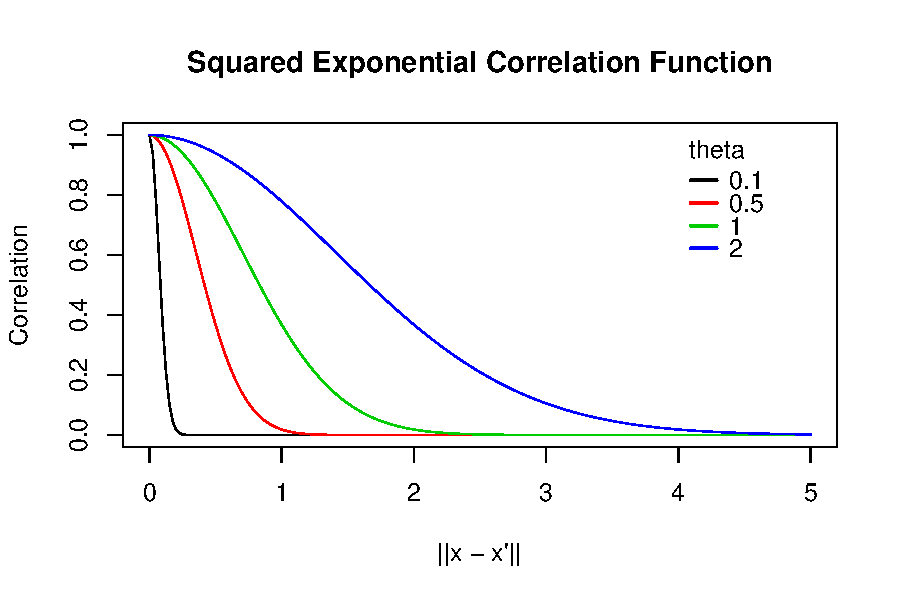
\includegraphics[width=\textwidth]{fig-emulators/squexp.pdf}
  \caption{Plot showing how $\theta$ affects the rate of decay of the correlation between model outputs as a function of the distance between inputs.}
  \label{Fig:sqexp}
\end{figure}
\begin{figure}[h]
  \centering
  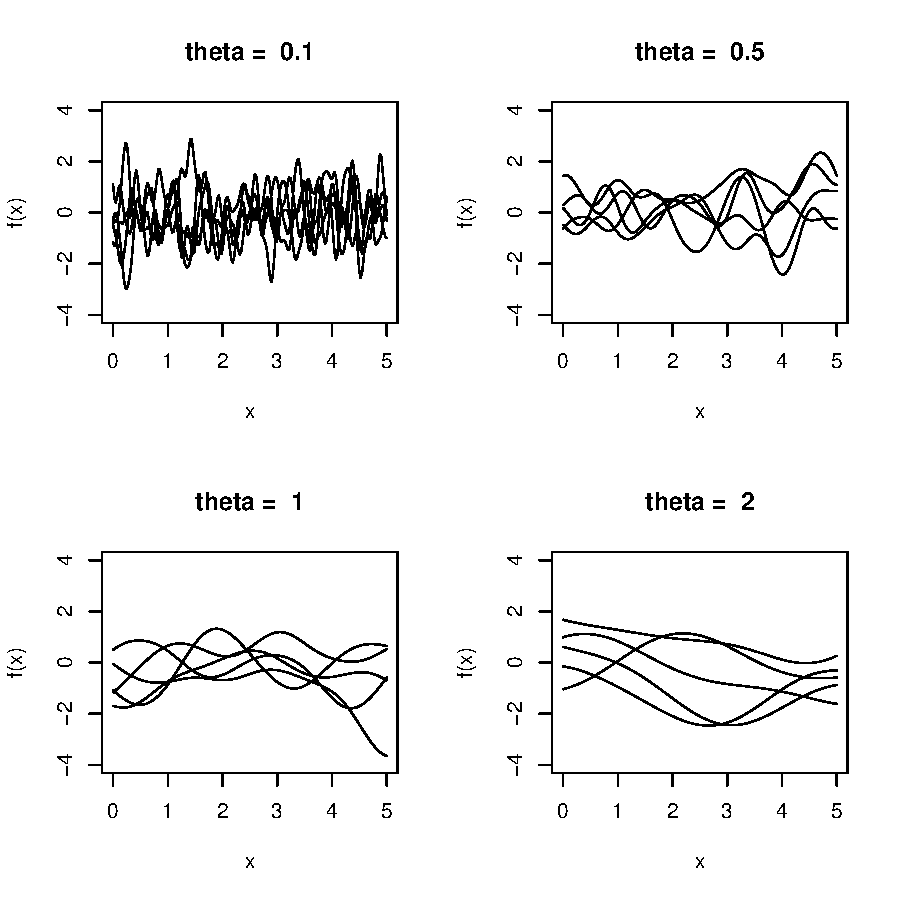
\includegraphics[width=\textwidth]{fig-emulators/random-func.pdf}
  \caption{Draws from a GP prior with squared exponential covariance function ($\sigma^2 = 1$) for varying values of $\theta$. Larger lengthscales correspond to smoother functions.}
  \label{Fig:random-funcs}
\end{figure}
Note that, although small lengthscales lead to very wiggly functions, it can be shown that functions drawn from a GP with squared exponential covariance are infinitely mean square differentiable. This seems reasonable for the functions we will encounter later in this thesis. Note that, although each function is drawn randomly, each realisation from a GP represents a deterministic function. It is as if we were to randomly draw parameters of a fixed functional form. The precise form is unknown, but not inherently stochastic. These ``spaghetti plots'' are great for visualising \textit{joint} behaviour of function draws, but not very good at showing us the marginal behaviour. To do this, we can plot the prior mean and some chosen prior quantiles. In the case of a stationary covariance function, $C(x, x) = \sigma^2$ and because we assumed a zero mean GP the (prior) marginal behaviour is independent of $x$; $f(x) \sim  N(0, \sigma^2)$.

The squared exponential is a limiting case of the Mat\'ern covariance function, which can be used to generate functions with a finite number of derivatives:
\begin{equation}
  C(x, x') = \sigma^2 \frac{2^{1-\nu}}{\Gamma(\nu)} \left( \sqrt{2\nu}\frac{||x - x'||}{\rho} \right)^\nu K_\nu\left(\sqrt{2\nu}\frac{||x - x'||}{\rho} \right)
\end{equation}
where $\sigma$, $\rho$, $\nu > 0$ and $K_\nu$ is the modified Bessel function of the second kind. Functions drawn from this prior are differentiable $\lfloor \nu \rfloor$ times in the mean-square sense. Letting $\nu \to \infty$ recovers the squared exponential covariance function. Like the squared exponential covariance function, the Mat\'ern covariance function is a stationary covariance function.

Another common covariance function is the linear covariance function:

\begin{align}
  C(x, x') &= \begin{pmatrix}
    1&x
\end{pmatrix}
\begin{pmatrix}
  b_0 & \frac{b_1}{2} \\ \frac{b_1}{2} & b_2
\end{pmatrix}
\begin{pmatrix}
  1 \\ x'
\end{pmatrix} \\ \nonumber
  &= b_{0} + b_{1}(x + x') + b_2 x x'.
\end{align}
The linear covariance function depends explicitly on $x$ and $x'$, and not the distance between them. This makes it a non-stationary covariance function. We later show that the linear covariance function is strongly related to many useful mean functions.

The final covariance function we consider is the white noise covariance function. This is just
\begin{equation}
  C(x, x') = \lambda^2 \mathbb{I}(x = x')
\end{equation}
where $\mathbb{I}(x = x')$ is an indicator function of the form
\begin{equation}
  \mathbb{I}(x = x') = \begin{cases}
    1, & x = x'\\
    0, & \text{ otherwise.}
  \end{cases}
\end{equation}
This covariance function isn't differentiable \textit{anywhere}. It can be used to generate independent and identically distributed (iid) $\mathcal{N}(0, \lambda^2)$ random variables (RVs). It is not useful on its own for generating functions but does act as a useful device for modelling random variation exhibited by a stochastic simulators such as the Athena simulator

In the context of emulation, $\lambda^2$ is often called the `nugget' term. Throughout this thesis, we will use both $\sigma^2$ and $\lambda^2$ as variances of Normal distributions. Unless explicitly stated otherwise, $\sigma^2$ will be the marginal (prior) variance of $f(\bx)$ whereas $\lambda^2$ will be the variance of the nugget term.

\subsection{Combining Covariance Functions}

For many practical problems, we are interested in varying multiple function inputs simultaneously. We can make multiple input covariance functions by combining standard ones. To construct a squared exponential covariance function for a $K$ input GP we multiply $K$ univariate squared exponential covariance functions:
\begin{equation}
C(\bx, \bx') = \sigma^2 \exp\left\{ - \sum_{i = 1}^K \frac{(x_i - {x_i}')^2}{\theta_i^2}\right\}.
\end{equation}
From hereon in, $\bx$ is a $K \geq 2$ dimensional input vector. Whenever we use $x$ this corresponds to a scalar input. This covariance function will take a large value when all the pairwise distances are small; it takes just one of the differences to be very large for the simulator outputs to be modelled as almost uncorrelated. If $\theta_i = \theta$ for each $i$ this is an \textit{isotropic} covariance functions. Otherwise, the covariance function is \textit{anisotropic}.

Adding covariance functions creates functions with different layers of complexity. One thing we might want to do is construct a function with a linear trend but allow for some variability around this trend. This is done by adding linear and (say) squared exponential covariance functions together. It can be seen in \Cref{Fig:mix-kern} that the resulting functions are roughly linear, but also feature some non-linear variation. In a regression context, this is useful when the data being modelled have an approximately linear trend but also some variation which is more difficult to describe.
\begin{figure}[h]
  \centering
  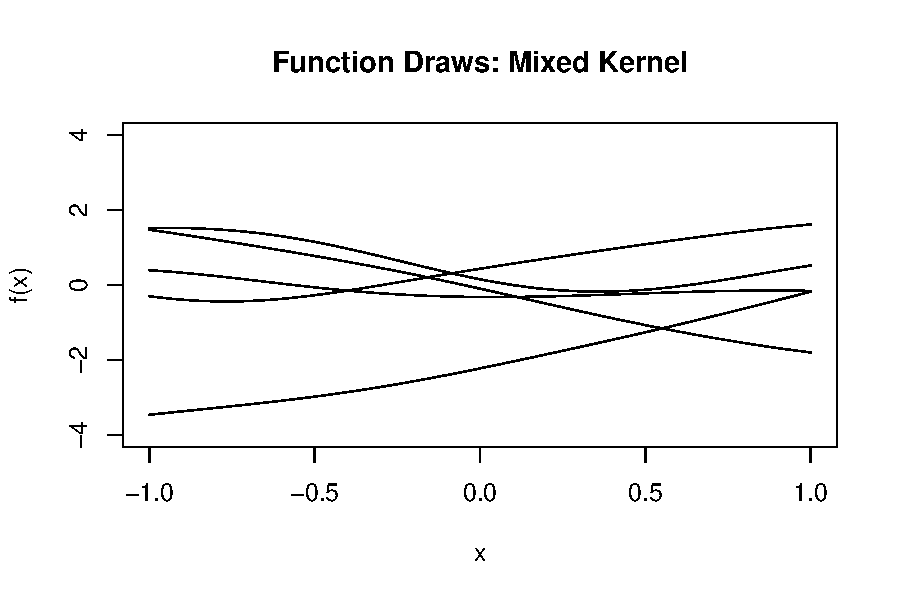
\includegraphics{fig-emulators/mixed-draws.pdf}
  \caption{Some realisations of a GP with linear $+$ squared exponential covariance function.}
  \label{Fig:mix-kern}
\end{figure}

\subsection{Mean Functions}

The simplest mean function is $\mu(\bx) = 0$ which corresponds to the GP being ``all covariance''. GPs can work really well in this case. Generalising to $\mu(\bx) = \beta$ centres the predictions around a more useful value, but again, this is a pure covariance approach after centring the data. It is frequently more useful to use mean functions which depend on $\bx$ and then use a zero mean GP to model variation about this systematic mean function. That is, write the model output
\begin{equation}
  f(\cdot) \sim \mathcal{GP}(\mu(\cdot), C(\cdot, \cdot))
\end{equation}
A popular approach is to construct the mean function hierarchically
\begin{equation}
  \mu(\bx) = h(\bx)^T \bm{\beta}
\end{equation}
where $h(\bx)$ is a $p$-vector with each element taking a simple, deterministic form and $\bm{\beta} = (\beta_0, \beta_1, \ldots, \beta_{p-1})^T$ are unknown regression coefficients to be inferred. A common form is $h(\bx)^T = (1, \bx)$. This expresses the belief that the function is approximately linear in its inputs. Some authors are proponents of using a very simple mean functions (constant, or zero), allowing the covariance structure to do the heavy lifting \citep{Henderson09,Zhang2019}. Some prefer a complex mean function which accounts for a large amount of variability in $f(\cdot)$ and using the GP to mop up the residuals. Providing the chosen mean function is sensible, this offers robustness against an inappropriate choice for $C(\cdot, \cdot)$ and can make the emulator more interpretable \citep{Xu16,Vernon2010}. This thesis generally takes a Goldilocks approach; the mean function should aim to capture the main global trends in $f(\bx)$ without being complicated. This can require much less effort than using  a complex mean function but despite the simplicity provides good results in many cases \citep{Ohagan01, Fricker2013, Fisher2021}. A different approach is to choose a complex mean form but use a prior that encourages sparsity amongst $\bm{\beta}$ to automatically choose a mean function \citep{Seshadri2020}.

\section{A General Gaussian Process Posterior}

\subsection{Parameter Inference}
Inferring the coefficients of the mean function and the parameters of the covariance function can be done in a frequentist or Bayesian way. If useful prior information is available, \citet{Oakley2002} describes how we might elicit $\mu(\cdot)$ (as well as the covariance structure). Suppose we have some data from the simulator. In this case, data are set of simulator inputs and corresponding outputs. That is $\mathcal{D} = \{ (y_i, \bx_i), i = 1, 2, \ldots, n \} $ where $y_i = f(\bx_i) + \varepsilon(\bx_i)$ and $\varepsilon(\bx_i) \sim N(0, \lambda^2(\bx_i))$ models inputs dependent noise in a stochastic simulator. Note that setting $\lambda^2(\bx) = \lambda^2$ recovers a constant level of noise and  $\lambda^2(\bx) = 0$ recovers a deterministic function. For now we will assume that $\lambda^2(\bx) = \lambda^2 \geq 0$. Even if theoretically we should take $\lambda = 0$, because the simulator is deterministic, it is computationally desirable to set $\lambda$ to be some small value (say $\lambda = 10^{-6}$) to avoid computational issues surrounding matrix inversion. Some authors support estimating $\lambda$ even when the simulator is deterministic as a way to account for assumptions such as stationary or the choice of covariance being incorrect \citep{Gramacy12}. This approach is not infallible; \citet{Andrianakis2012} show this can lead to problems such as (i) bimodal likelihoods and (ii) ill-fitting emulators.

Regardless of whether the simulator is stochastic or deterministic, the likelihood function is then
\begin{equation}
  \by \mid \bm{\beta}, \Theta \sim \mathcal{N} \left\{ H\bm{\beta}, \Sigma\right\}
\end{equation} where $H$ is the design matrix with $j$th row $h^T(\bx_j)$ where $\bx_j$ is the $j$th vector of simulator inputs, $\Sigma = C(X, X) + \lambda^2 I$ and $\Theta$ are the parameters of the covariance function. Assuming a squared exponential covariance function, and a nugget term, leads to $\Theta = (\sigma, \theta_1, \theta_2, \ldots, \theta_K, \lambda)$.  In a Frequentist framework, we can maximise like likelihood to obtain estimates $\hat{\bm{\beta}}$ and $\hat{\Theta}$ \citep{Sacks89}. In a Bayesian framework we could elicit a prior $\pi(\bm{\beta}, \Theta)$ then use MCMC to obtain samples from $\pi(\bm{\beta}, \Theta \mid \mathd)$ \citep{Svalova2021}. Alternatively,  we can maximise the posterior density to obtain \textit{maximum a posteriori} (MAP) estimates \citep{Baker2020a}. It is desirable, for computational reasons, to analytically integrate out parameters where possible. If we take $\bm{\beta} \sim \mathcal{N}(\bm{b}, B)$ this is possible. Following \citet{BDA3} (see appendix A of the reference), and noting that $\var\{H\beta\} = H^T B H$, it can be shown that we can write the distribution of $\by \mid \Theta$ as
\begin{equation}
  \by \mid \Theta \sim \mathcal{N} \left\{ H \bm{b}, \Sigma + H^T B H\right\}. \label{Eq:int-mean}
\end{equation}
   Now inference about $\Theta$ follows by treating \Cref{Eq:int-mean} as a likelihood function. This reduced parameter space can lead to faster inferences. From this we can obtain MLE/MAP estimates or perform a full Bayes analysis. Note that if we take $\pi(\bm{\beta}, \sigma \mid \bm{\theta}, \lambda) \propto \sigma^{-2}$ (i.e. implying infinite prior variance on $\bm{\beta}$) then both $\bm{\beta}$ and $\sigma$ can be analytically integrated out. The resulting emulator is a Student's $t$ process \citep{Oakley2002a}.
\subsection{Posterior Predictive Distribution}
A GP prior on $f(\cdot)$, $\pi(f(\cdot))$, is infinite dimensional, as is the posterior, $\pi(f(\cdot) \mid \mathcal{D})$. Both of these facts are due to there being an infinite number of choices for $\bx$. Luckily, this issue can be sidestepped we can easily find $\pi(f(X^*) \mid \mathcal{D})$ for any finite collection of inputs, $X^*$. In practice this is enough to allow us to perform any task that we would use $f(\cdot)$ for.

Now assume a mean function of the form $\mu(\bx) = h(\bx)^T \bm{\beta}$. Consider a collection of simulator outputs $\by^{(1)} = (y_1^{(1)}, y_2^{(1)}, \ldots, y_n^{(1)})^T$ at inputs
\begin{equation}
  X^{(1)} = \begin{pmatrix} \bx_1^{(1)} \\ \bx_2^{(1)} \\ \vdots \\ \bx_n^{(1)} \end{pmatrix}
\end{equation} and let the corresponding design matrix be $H_1$. We want to infer $\by^{(2)} = (y_1^{(2)}, y_2^{(2)}, \ldots, y_m^{(2)})^T$, the outputs at $X^{(2)}$ with corresponding design matrix $H_2$. After integrating out $\bm{\beta} \sim \mathcal{N}\{ \bm{b}, B\}$, we are left with the following relationship between the two sets of simulator outputs:
\begin{equation}
  \begin{pmatrix}
    \by^{(1)} \\ \by^{(2)}
  \end{pmatrix} \mid \Theta \sim \mathcal{N} \left\{
   \begin{pmatrix}
    H_1 \bm{b} \\ H_2 \bm{b}
  \end{pmatrix}, \begin{pmatrix} K(X^{(1)}, X^{(1)}) & K(X^{(1)}, X^{(2)}) \\
K(X^{(2)}, X^{(1)}) & K(X^{(2)}, X^{(2)}) \end{pmatrix} \right\}.
\end{equation}
where $K(X^{(i)}, X^{(j)}) = C(X^{(i)}, X^{(j)}) + H_i B H_j^T + \lambda^2 \mathbb{I}(i = j)$. Unless explicitly stated, $C(\cdot, \cdot)$ is used for squared exponential covariance functions and $K(\cdot, \cdot)$ represents the addition of a squared exponential and linear covariance functions and possibly a nugget term.

Then the posterior predictive distribution for $\by^{(2)}$ is also multivariate Normal \citep{Rasmussen2006Gpfm}. The mean and variance are as follows:
\begin{align}
  \E \left\{ \by^{(2)} \mid \Theta, \mathd \right\} &= H_2 \bm{b} + K(X^{(2)}, X^{(1)})K(X^{(1)}, X^{(1)})^{-1} \left( \by^{(1)} - H_1 \bm{b} \right) \label{Eq:MV1}\\
  \var \left\{\by^{(2)} \mid \Theta, \mathd \right\} &= K(X^{(2)}, X^{(2)})- K(X^{(2)}, X^{(1)})K(X^{(1)}, X^{(1)})^{-1}K(X^{(1)}, X^{(2)}).\label{Eq:MV2}
\end{align}
Observing the form of the equations we can see that the posterior mean is just the prior mean with an adjustment based on how far the prior form is from the observed outputs. The size of that adjustment depends on how well the prior model fits the observed data and how correlated we expect $\by^{(1)}$ and $\by^{(2)}$ to be. The posterior variance is always \textit{less than} the prior variance and, surprisingly, is independent of the observed $\by^{(1)}$.  The posterior variance depends only on the locations of simulators inputs we are interested in and their distances from the design points. However, if $\Theta$ is inferred, rather than specified, then there is a dependence on $\by^{(1)}$ via the likelihood function. Throughout this thesis, we will often refer to the ``conditional Normal equations'' which means equations with the same form as \Cref{Eq:MV1} and \Cref{Eq:MV2}. For brevity, we will denote the posterior mean at input $\bx$ by $m^{*}(\bx)$ and posterior variance at $\bx$ by $v^{*}(\bx)$.

\subsection{Specific Examples}

 We will now observe how aspects of a GP prior impact the posterior. We will focus on squared exponential, linear, and white-noise covariances. We will fit an emulator to a simple, tractable example to allow us to easily compare the fit to the truth. We will work with
 \begin{equation}
   f(x) = 2 \sin (2 \pi x) + \cos(3\pi x) + 3x. \label{Eq:toy-fn}
 \end{equation}
In a more realistic scenario, the simulator is described by complex mathematical equations and implemented via many lines of computer code, thus the exact functional form is not known. We will assume a linear trend with prior mean $\E (\beta) = \bm{0}$ and $\var(\bm{\beta}) = 2I_2$ where $I_k$ is the $k \times k$ identity matrix. Using $n = 10$ design points chosen by uniform sampling and a squared exponential covariance function with $\sigma = 3$ and $\theta = 0.5$ we can calculate the posterior distribution for any $x$ via the conditional Normal equations.
\begin{figure}[h]
  \centering
  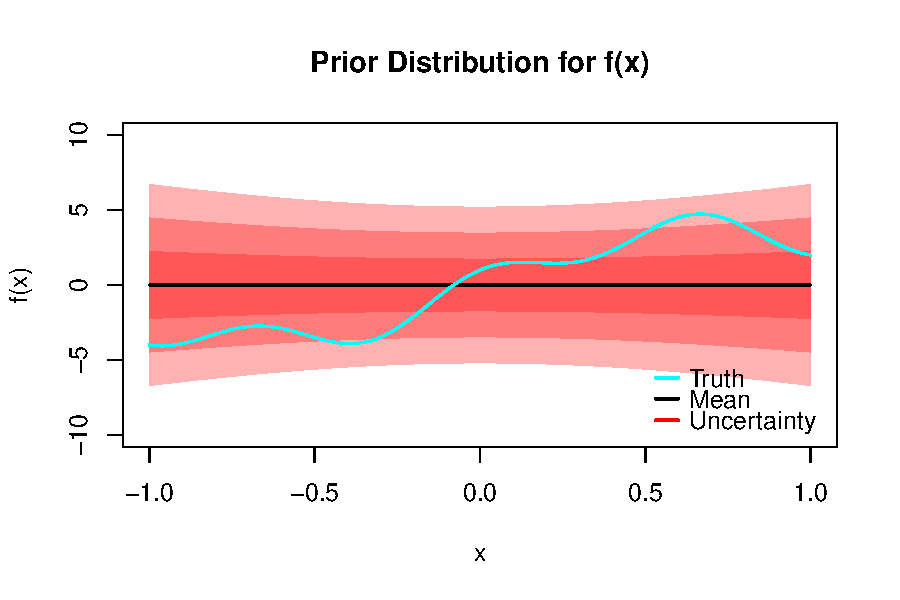
\includegraphics{fig-emulators/prior.pdf}
  \caption{Our prior specification for the simulator specified by \Cref{Eq:toy-fn}. The simulator is shown as the blue line, emulator prior mean as the black line and uncertainty is represented by the red bands; $\mu(x) \pm (1,2,3)\sqrt{K(x,x)}$.}
  \label{Fig:prior}
\end{figure}
\begin{figure}[h]
  \centering
  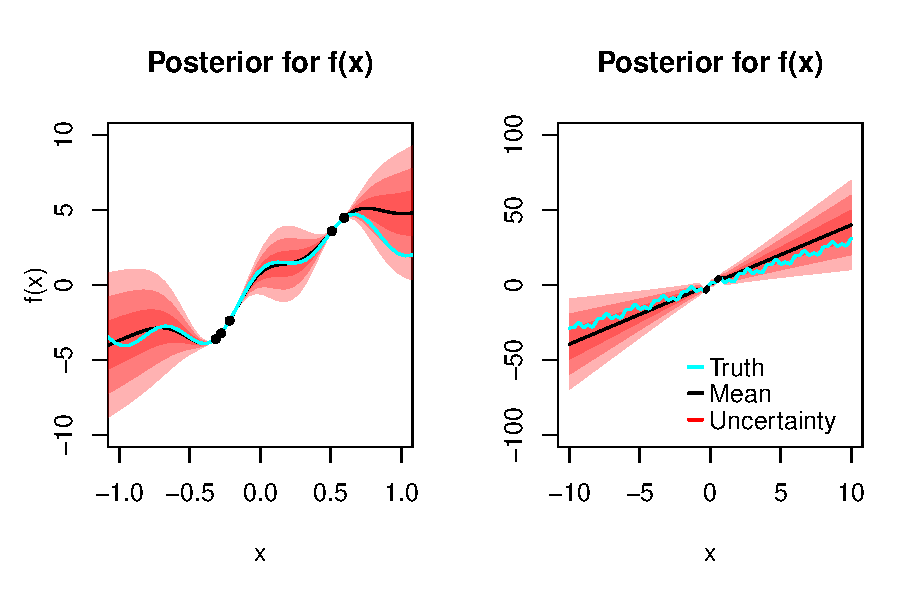
\includegraphics{fig-emulators/dual-posterior.pdf}
  \caption{The posterior distribution for the simulator specified by \Cref{Eq:toy-fn}. The simulator is shown as the blue line, the emulator posterior mean as the black line and posterior uncertainty is represented by the red bands; $m^{*} (x) \pm (1,2,3)\sqrt{ v^{*}(x) } $. The left hand plot shows how the emulator captures local variation in $f(\cdot)$ whereas the right hand plot illustrates the estimated global variation.}
  \label{Fig:posterior}
\end{figure}

An interesting feature of our prior (\Cref{Fig:prior}) is that the width of the prior predictive interval depends on $x$. Some interesting features of GP posteriors are:
\begin{itemize}
  \item[(i)] $v^* (x) = 0 \text{ and } m^*(x) = f(x) \iff x$ is a training point and $\lambda = 0$
  \item[(ii)] $v^* (x)$ is small when $x$ is close to a training points
  \item[(iii)]  When $x$ is far from the training data, $m^*(x) \approx h(x)^T \E \{ \bm{\beta} \mid \mathd \} $.
  \item[(iv)] When $x$ is far from the training data, $v^*(x) \approx K(x,x)$.
\end{itemize}
A ``proof'' by picture of these properties is given in the the plotted posterior distribution of the synthetic example (\Cref{Fig:posterior}). The uncertainty is very small close to the training points and the mean function is close to the function values (a computational nugget $\lambda^2 = 10^{-6}$ was used here), this illustrates (i) and (ii). When we are far from the training data, the width of our posterior uncertainty bands is close to that of our prior uncertainty bands. \Cref{Fig:posterior} (left) does not clearly illustrate properties (iii) and (iv). Zooming out gives the right hand plot and shows shows that the expected response is linear when $x$ is far from the training data.

\subsection{Stochastic Computer Simulators}

It is straightforward to extend emulators to stochastic computer models. That is, those exhibiting random variation. A feature of these models is that runs of the simulator return different values even if $\bx$ remains unchanged. Our motivating example, Athena, is stochastic. This approach to simulation allows us to investigate two major sources of uncertainty:
\begin{itemize}
  \item[(i)] the stochastic nature of the world (aleatory uncertainty)
  \item[(ii)] randomising inputs to account for lack of knowledge (epistemic uncertainty).
\end{itemize}
Aleatory uncertainty is a desirable feature of models where the response is ultimately difficult to predict. For example, in the Athena simulator, aspects of the simulator are random to account for difficult to predict features such as weather and human error. Accounting for epistemic uncertainty is achieved by assigning a probability distribution to a some (or all) input parameters and propagating this uncertainty through $f(\cdot)$, usually with the help of an emulator \citep{Oakley04}.

Under stochasticity we need to be careful about what we want to infer, and hence we will be careful with our notation. Let $y(\bx)$ be the simulator output at $\bx$ and let $f(\bx)$ be the mean response at $\bx$. Under the GP framework, we perform inference on $f$ and $y$ simultaneously. We can specify their relationship hierarchically,
\begin{align}
  y(\bx) \mid f(\bx), \lambda^2, \Theta, \bm{\beta} &\sim \mathcal{N}(f(\bx), \lambda^2) \label{Eq:homgp1} \\
  f(\cdot)  \mid \Theta, \bm{\beta} &\sim \mathcal{GP} \{ h(\cdot)^T \bm{\beta}, C(\cdot, \cdot) \}.\label{Eq:homgp2}
\end{align}
Now, since iid $N(0, \lambda^2)$ noise is equivalent to the white noise covariance structure, we can integrate out $f(\cdot)$ and $\bm{\beta}$. This leads to
\begin{equation}
  y(\cdot) \mid \Theta \sim \mathcal{GP}\left\{ h(\cdot)^T\bm{b}, K(\cdot, \cdot) + \lambda^2 I \right\}
\end{equation}
where $h(\cdot)$ and $K(\cdot, \cdot)$ have their usual meanings. Prediction of the mean function is exactly the same as in \Cref{Eq:MV1}. Posterior variances of $y(X^*)$ and $f(X^*)$ differ only by $\lambda^2$:
\begin{align}
  \var(f(X^*) \mid \mathd, \Theta) &= K(X^*, X^*) - K(X^*, X) V^{-1} K(X, X^*)\label{Eq:vary} \\
  \var( y(X^*) \mid \mathd, \Theta) &= K(X^*, X^*)  + \lambda^2 I - K(X^*, X) V^{-1} K(X, X^*).\label{Eq:varf}
\end{align}
where $V = K(X, X) + \lambda^2 I$. \Cref{Eq:varf} allows us to make statements about $f(\bx)$ and \Cref{Eq:vary} allows us to make statements about $y(\bx)$. The difference between them is analogous to the difference between a confidence interval, and a prediction interval in a frequentist regression analysis.
The properties (i) and (ii) of GP posteriors don't hold here because $\lambda$ may be arbitrarily large to account for arbitrary amounts of stochasticity. Good prior information, usually specified via the mean function, can be very important in the stochastic setting since, especially if $\lambda$ is large, $\by(X)$ might not be very informative for $f(X)$. We demonstrate this by adapting \Cref{Eq:toy-fn} to be stochastic. We introduce stochasticity by simulating from $y(\bx) \sim \mathcal{N} \{f(\bx), 0.5^2 \}$. This can be seen in \Cref{Fig:toy-stoch}. There is still a fairly large amount of uncertainty close to the design points. An infinite sample size is required for this uncertainty to reduce to zero. The probability bands for $y(x)$ take into account uncertainty about $f(x)$ as well as stochasticity.
\begin{figure}[h]
  \centering
  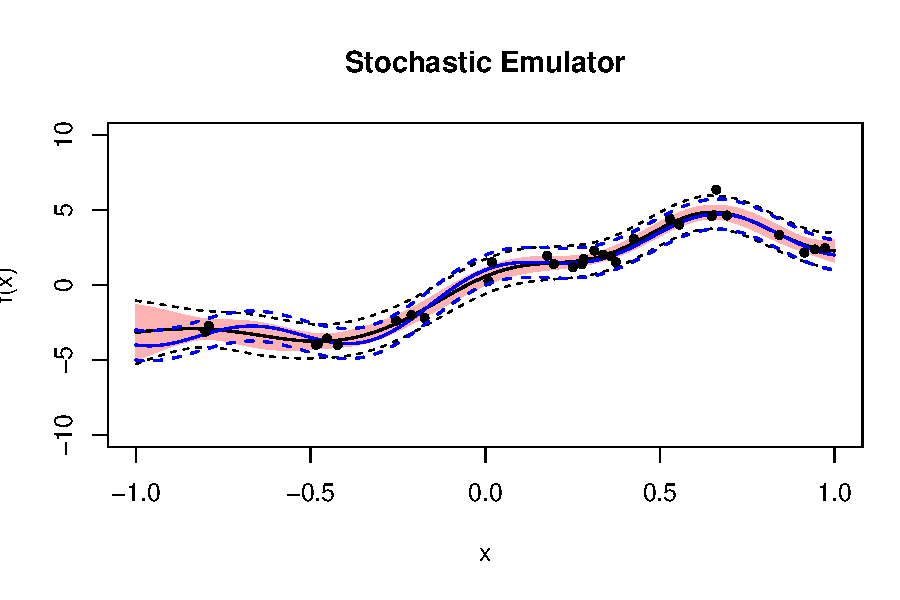
\includegraphics[width = \textwidth]{fig-emulators/toy-stoch.pdf}
  \caption{An emulator for a stochastic simulator. Solid blue line is simulator mean with blue dashed lines being $95\%$ probability bands. Solid black line is emulator mean, dashed black lines are a $95\%$ probability interval for $y(x)$ and the red band is a $95\%$ probability interval for $f(x)$.}
  \label{Fig:toy-stoch}
\end{figure}
\section{Design for Computer Experiments}
The previous figures in used a simple uniform sample for selecting locations at which to run the simulator. In practice, this is usually a bad idea since uniform designs can often lead to design points which are very close together in space. This somewhat wasteful since our smoothness assumptions about $f(\cdot)$ imply that $||f(\bx) - f(\bx')||$ is small whenever $||\bx - \bx'||$ is small. It therefore makes sense to spread out the design points where possible. Such designs are termed ``space filling'' designs.
Another design approach is to sequentially construct the emulator. This involves using the emulator, combined with a rule, $\alpha(\bx)$, to choose where to next run the simulator. The simulator is then run at the point satisfying $\bx^\star = \argmax_{\bx \in \mathcal{X}} \alpha(\bx)$, the emulator is updated and we repeat the process until we satisfy some stopping rule.
In general, there is no globally superior choice as to whether we go with one-shot or sequential designs, and a sequential design may be initialised by a small one-shot design \citep{Zhang2019}. One-shot designs are typically easier and cheaper to implement than sequential designs. We construct the design and run the simulator in isolation of each other. Sequential designs need the simulator and emulator to `talk' to each other, which might be difficult if the person constructing the emulator is not familiar with the language the simulator is implemented in. The final advantage of one-shot designs is that there is no connection to the final form of the emulator (e.g. they are agnostic to choice of covariance and mean functions and allow us to drop inputs from the emulator that were included in the simulator). For instance, \citet{Overstall2017} use a single one-shot design to construct and compare many emulators based on just one training set and one validation set. On the other hand, sequential designs can leverage our current understanding of $f(\cdot)$ (or $y(\cdot))$ to achieve specific goals more efficiently that a one-shot approach. A popular class of sequential designs, Bayesian Optimisation acquisition functions \citep{Frazier2018}, are those which aim to optimise $f(\cdot)$ whilst minimising the number of times we run the simulator.
\subsection{One-Shot Designs}
Perhaps the most popular one-shot designs in the computer experiments literature are Latin Hypercube (LH) designs. A LH, of size $n$, of dimension $K$, is constructed by partitioning the sample space into $n$ equally sized $K$-dimensional hypercubes and a singe uniform sample is taken from each sub-hypercube. This leads to a `more uniform' design than truly uniform sampling. This construction allows us to guarantee that for a LH of size $n$, in each margin, there is exactly $1$ sample in each interval. This shows a clear advantage over pure uniform designs. In \Cref{Fig:rand-lh} we see a particularly unfortunate uniform design in which no samples appear above the line $x_1=x_2$ and most of the points satisfy $x_2 < 0.2$. The LH offers some protection against this, but is not watertight. For example, sampling amongst the diagonal boxes would lead to a valid LH design, but not a space filling design.
\begin{figure}[h]
  \centering
  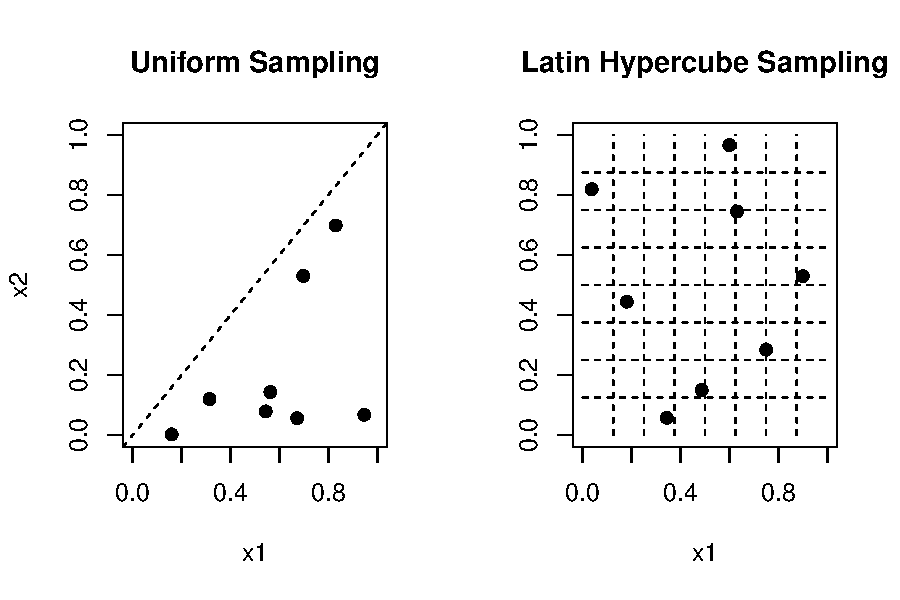
\includegraphics{fig-emulators/rand-latin.pdf}
  \caption{A $2$d random sample (left) and $2$d LH sample (right), both of size $n = 8$. In the left plot the dashed line corresponds to unit diagonal, in the right the dashed lines correspond to an $8 \times 8$ grid of equally sized sub-cubes.}
  \label{Fig:rand-lh}
\end{figure}
We can enhance LHs with additional structure to obtain a more space filling design. One such enhancement is the maximin LH. A maximin design is one which maximises the minimum distance between design points so that no pair of points are too close. This rule can be added to a LH to prevent the points sitting on the diagonal or for two points to be sitting in nearby corners of adjacent sub-cubes \citep{Mckay1979, Morris1995}.
\subsection{Sequential Designs}
As discussed, sequential designs allow us to leverage our current state of knowledge to satisfy some optimallity criterion. Many such designs are Bayesian since they can be expressed as expectations of random variables. For example, consider Active Learning McKay (ALM), which is based on posterior variance (and recall, the variance is the expected squared distance from the mean) \citep{Seo2000}. If we have already run the simulator at $n$ locations, then the next point to run the simulator at, $\bx_{n+1}$, is given by
\begin{align}
  \bx_{n+1} &= \argmax_{\bx \in \mathcal{X}} \alpha_{ALM}(\bx)\\
    \alpha_{ALM}(\bx) &= v^{*}(\bx)
\end{align}
That is, we run the simulator at the location with largest uncertainty (about the underlying mean) in the design space $\mathcal{X}$. The idea here is to reduce uncertainty to construct a globally accurate emulator. An approach with similar goals is to minimise the integrated mean square prediction error (IMSPE), which is given as
\begin{equation}
  \alpha_{IMSPE}(\bx) =  -  \int_{\tilde{\bx} \in \mathcal{X}} \left\{ y(\tilde{\bx}) - m^* (\tilde{\bx}) \right\} ^2 \dd \tilde{\bx}.
\end{equation}
IMSPE aims to minimise the average uncertainty across $\mathcal{X}$ rather than point-wise uncertainty. This is probably a more desirable tactic than ALM, however is requires integration over $\mathcal{X}$ which can be a tricky task \citep{Gramacy2020surrogates}.
\section{Model Fidelity}
In many scenarios, the simulator of interest can be run at varying levels of complexity. The complexity induces a trade-off between the accuracy of simulations and the corresponding computational cost. `Cost' usually means wall clock computation time, but this could be generalised to say financial cost if high performance computing facilities are hired to obtain training data.
There are two main methods for constructing emulators in this scenario. One is a cumulative roughness model in which the cheapest code `level' is thought to be relatively smooth and more expensive levels are thought to have a rougher, more complex response surface. The more common type is an autoregressive model, which has strong links to co-Kriging in the geostatistics literature \citep{Stein1991}. Both of these methods go by multiple names including `multilevel emulation', `multifidelity emulation' or some use co-Kriging regardless of whether the approach is used in geostatistics or emulation.

The core idea in both multilevel emulation and co-Kriging is that using a large, auxiliary data set, can help fill in the gaps of a sparse data set of direct interest. In geostatistics, we might have a small number of expensive, but highly accurate weather sensors placed over an area of interest. We may also have a much larger number of cheap, but inaccurate sensors placed over the same area. The cheap sensors provide a prediction of what the expensive sensors would report. We then construct a GP regression model based on the readings from cheap sensors but then perform a correction based on the expensive readings to provide an improved prediction of the weather at locations without a weather sensor. See \citet{Yates1987,Ashraf1997,Lark2007,Adhikary2017} for various examples.
This concept can be adapted to the emulation literature. In many cases, accuracy is increased by making a time step in a differential equation solver smaller, or by constructing finer grids over space in spatial type models. Another scenario would be where there are two separate models; a cheap model with simple physics and an expensive model with much more complex physics.
Two methods of combining runs from these these different, but related, simulations are proposed by \citet{Kennedy2000}. Both models then become more accurate in the sense that they are better approximations of the mathematical equations being solved, they are not necessarily better approximations to reality.
\subsection{Autoregressive Models}
A common approach to modelling simulators of different accuracy is via an autoregressive structure. Suppose we have a simulator $f_t(\bx)$ where $t \in \{1, 2, \ldots, T\}$ are the simulator levels. If $s>t$ then then $f_s(\cdot)$ is assumed to be more accurate but also more expensive to run than $f_t(\bx)$. We assume that we have $n_t$ runs of each simulator where $s > t$ implies that $n_s < n_t$. We can then induce the following model on the simulators:
\begin{align}
  f_1(\cdot) \mid \bm{\beta}_1, \Theta_1 &\sim \mathcal{GP}(h(\bx)^T \bm{\beta}_1, c_1(\cdot, \cdot))\\
  f_{t+1}(\cdot) \mid f_{t}, \bm{\beta}_{t+1}, \Theta_{t+1}&= \rho_{t}f_{t}(\cdot) + \delta_{t+1} (\cdot)
\end{align}
where $\delta_t(\cdot) \sim \mathcal{GP}\left\{h(\cdot)^T\bm{\beta}_t, C_t(\cdot, \cdot) \right\}$ and $\Theta_t$ are the hyperparameters of $c_t(\cdot,\cdot)$ and $\rho_t$ describes how correlated $f_t(\bx)$ and $f_{t+1}(\bx)$ are. The term $\delta_{t+1}(\cdot)$ essentially represents the discrepancy between $f_t(\cdot)$ and $f_{t+1}(\cdot)$. This model relies on $f_t(\cdot)$ explaining most of the variation in $f_{t+1}(\cdot)$. It is then assumed that the $\delta_t(\cdot)$ processes are much simpler than the corresponding $f_t(\cdot)$.
If we take \begin{equation}
  c_t(\bx, \bx') = \sigma_t^2 \exp \left\{ - \sum_{i = 1}^K \frac{(x_{i} - {x_i}')^2}{\theta_{t,i}^2} \right\}
\end{equation} it then follows that \begin{equation}
  \cov(f_t(\bx), f_{t+1}(\bx')\mid \bm{\beta}, \Theta) = \rho_t \sigma_t^2 \exp \left\{ - \sum_{i = 1}^K \frac{(x_i - {x_i}')^2}{\theta_{t,i}^2} \right\}.
\end{equation}
where $\bm{\beta} = \{\bm{\beta}_1, \bm{\beta}_2, \ldots, \bm{\beta}_T\}$ and $\Theta = \{\Theta_1, \Theta_2, \ldots, \Theta_T\}$.
The design of these multilevel experiments is interesting. \citet{Kennedy2000} shows that the likelihood is greatly simplified if $D_{t+1} \subset D_t$, that is, we run $f_{t+1}$ only at the locations which $f_t$ has been run. Rather than fitting one joint model, this allows us to fit a GP to $f_1(\cdot)$ and then to each $\delta_t(\cdot)$. In such a case, the design matrix is of the form
\begin{equation}
  H = \begin{pmatrix}
    h(X_1) & \bm{0} & \cdots & \bm{0} & \bm{0}) \\
    \rho_{(1,1)} h(X_1) & h(X_2) & \cdots & \bm{0} & \bm{0}\\
    \vdots & \vdots & \ddots & \vdots & \vdots\\
    \rho_{(1, T-1)} h(X_1) & \rho_{(2, T-1)}h(X_2) &\cdots &\rho_{(T-2, T-1)}h(X_{T-1}) & h(X_T)
\end{pmatrix}.
\end{equation}
where $\rho_{(t, s)} = \prod_{i = t}^s \rho_i$ for $s>t$. Further, conditional on all GP parameters, the covariance function for $f_t(\cdot)$ ($t \geq 2$) is
\begin{equation}
  C_t(\bx, \bx') = c_t(\bx, \bx') + \sum_{j = 1}^{t-1} \rho_{(1, j)}^2 c_j(\bx, \bx').
\end{equation}
\subsubsection{A Tractable Example}
Consider the computation of the following integral, which is viewed as a function of $x$:
\begin{equation}
  f(x) = \int_0^1 \cos(4 \pi x^2)\sin(2 \pi xt) - 4xt + 1 \diff t.
\end{equation}
This is an easy to compute integral, but if the integral was intractable, this could be replaced by a Riemann approximation:
\begin{equation}
  f_R(x; T) = \sum_{i = 0}^{T-1} g(t_i ; x).
\end{equation}
where $g(t ; x) = \cos(4 \pi x^2)\sin(2 \pi t x) - 4xt + 1$ is the integrand and $t_i = \tfrac{i}{T-1}$ are the equally spaced points at which $g(t;x)$ is evaluated. This integrand is cheap but in a complex computer model could be expensive to evaluate. \Cref{Fig:fidelity} shows how increasing the number of evaluations of $g(t;x)$ improves the approximation. We see for $T=2$ the approximation is bad; there is a phase-shift. For $T \geq 4$ the approximation improves, but with diminishing returns.
\begin{figure}[h]
  \centering
  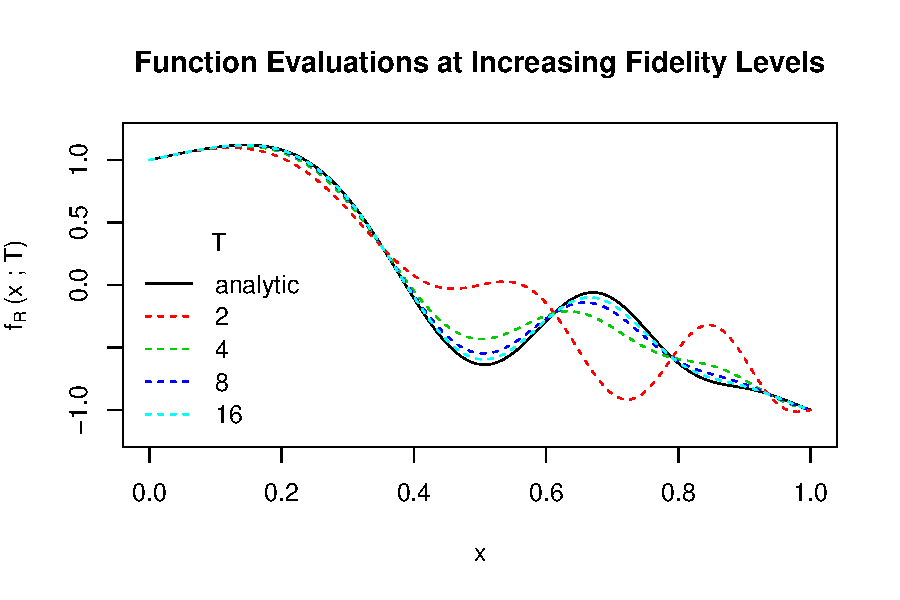
\includegraphics{fig-emulators/fidelity.pdf}
  \caption{Solutions to $f_R(x;T)$ at different fidelity levels. Approximate solutions are given by dashed lines, the analytic solution is given by the solid line. $T$ corresponds to the number of evaluations of $g(t;x)$ in the Riemann integration.}
  \label{Fig:fidelity}
\end{figure}
Suppose we have $n_e = 3$ evaluations of $f_R(x; 40)$ but also have $n_c = 20$ evaluations of $f_R(x;4)$. The evaluations of $f_R(x;4)$ may have been from a trial, exploratory run of the simulator or chosen to help inform us about $f_R(x; 40)$.
\begin{figure}[h]
  \centering
  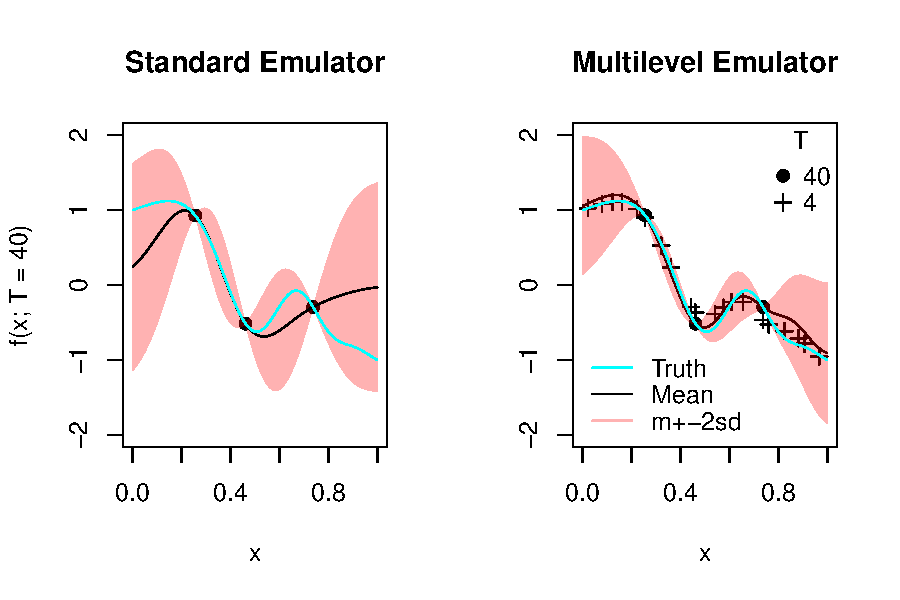
\includegraphics{fig-emulators/compare-ml.pdf}
  \caption{A standard GP emulator (left) and corresponding multilevel emulator (right). Here, the `truth' refers to $f_R(x;40)$, the object of inference, rather than the analytic solution.}
  \label{Fig:compare-ml}
\end{figure}
We see, qualitatively, that the multilevel emulator offers an improved fit over the standard emulator (\Cref{Fig:compare-ml}). Firstly, the mean function more closely reflects the truth, this is especially noticeable once we start extrapolating beyond the range of the observed expensive data. There is also a moderate reduction in uncertainty about the expected function value, reflecting that the auxiliary information from a different level of code \textit{is} informative for a more expensive version. In this toy, $1$-dimensional example, it is easy to see that the multilevel emulator is better.
\section{Emulator Comparison}
When fitting an emulator in a higher dimensional space, it is much trickier to assess fit. We will now demonstrate some emulator performance metrics on the standard GP and the multilevel emulator from \cref{Fig:compare-ml}. Here we consider the use of two performance metrics to assess the emulator. The first is root mean squared error (RMSE). Given a set of set of `unseen' data $\mathcal{D}_{\text{test}} = \{ (\bx_{\text{test},i}, y_{\text{test},i}), i = 1, 2, \ldots, n_{\text{test}} \} $, this can be found via
\begin{equation}
  RMSE = \sqrt{ \frac{1}{n_\text{test}}  \sum_{i = 1}^{n_\text{test}} \left\{ y_{\text{test},i} - m^*( \bx_{\text{test},i} )  \right\}^2 }. \label{Eq:rmse}
\end{equation}
All RMSE tells us is how close $m(\cdot)$ is to $f(\cdot)$. This doesn't take into account the uncertainty about $f(\cdot)$ or $y(\cdot)$, which motivates the use of a proper scoring rule. Proper scoring rules reward forecasts with high certainty when they are accurate but do not heavily penalise inaccurate forecasts when they have a large uncertainty attached to them \citep{Gneiting2007}. For GP emulators, the following scoring rule (bigger is better) is commonly used \citep{Binois2018,Jackson2019}
\begin{equation}
  S(\mathcal{D}_\text{test}) = -\frac{1}{n_{\text{test}}}\sum_{i = 1}^{n_\text{test}}\left\{ \frac{[y_{\text{test},i} - m^*(\bx_{\text{test},i} ) ]^2}{v^*(\bx_{\text{test},i})} + \log v^*(\bx_{\text{test},i})\right\}.\label{Eq:scoring-rule}
\end{equation}
\Cref{Eq:scoring-rule} is essentially the pointwise log-likelihood of a Normal distribution.
Returning to the multilevel emulators, we compute the RMSE and score for each emulator based on the two proposed metrics based on $100$ equally spaced test points. This is a very large number of test points relative to the design. In practice, the size of the test set would likely be no larger than the training design. There does not appear to be any literature on appropriate sizes for test designs, but types of design have been explored \citep{Challenor2013}.

\Cref{Tab:toy-ml-metric} gives the two pairs of performance metrics for the competing emulators. The RMSE for the multilevel emulator is much smaller than the standard emulator, this is expected since \cref{Fig:compare-ml} showed that the emulators mean for the multilevel emulator was almost the same as the target function. The score also shows a healthy improvement under the multilevel approach, this tells us that, in a combined sense, the posterior distribution provided by the multilevel emulator is a better probabilistic prediction than the posterior distribution provided by the standard emulator.
\begin{table}
\centering
  \begin{tabular}{rll}
    \toprule
    Emulator & RMSE & Score \\ \cmidrule{1-3}
    Standard&$0.4292$&$1.917$\\
    Multilevel&$0.1139$&$3.588$\\
    \bottomrule
  \end{tabular}
  \caption{Performance metrics for two the standard and multilevel emulators in \Cref{Fig:compare-ml}.}
  \label{Tab:toy-ml-metric}
\end{table}
\section{Emulator Diagnostics}
As with any statistical model, we must investigate whether the emulator is an appropriate approximation to the simulator. The main emulator diagnostics, for deterministic simulators, were proposed by \citet{Bastos09} (from hereon in, BO'H). A similar set of diagnostics have been proposed by \citet{Baker2019a} for stochastic simulators.
Here we review the diagnostics proposed by BO'H that are used later in this thesis. However, BO'H integrate out $\sigma$ in their emulators, resulting in the posterior being a Student's $t$ process. We will always conditions on $\sigma$, thus the posterior is Gaussian. Therefore, the diagnostics we present have been adapted to assume a GP posterior.
\subsection{The Diagnostics}
The diagnostics all rely on Cholesky Errors (C.E.s). These are analogous to standardised residuals in a standard regression analysis but take into account the covariance structure of the emulator. This is importance since, we expect $||f(\bx) - f(\bx')||$ to be small whenever $||\bx - \bx'||$ is small. In other words, we expect the residuals to have structure even when the emulator is an appropriate representation of the simulator. The C.E.s are defined to be
\begin{equation}
  \bm{e}_{\text{chol}} = \Sigma_\text{test}^{-1/2}(\by_{\text{test}} - m^{*}(X_{\text{test}}))
\end{equation}
where $m^*(X_{\text{test}})$ is the emulator's posterior mean vector and $\Sigma_\text{test}$ is the posterior variance matrix for the test points. $\Sigma^{-1/2}_\text{test}$ is the inverse of the lower Cholesky decomposition of $\Sigma_\text{test}$. If the emulator is an adequate approximation to the simulator then $\bm{e}_\text{chol}$ should appear as a random sample from $N_{n_\text{test}}(0, I)$ when plotted against $x_{\text{test},i}$. We can perform further diagnostics based on these residuals. Since they are (supposedly) a random sample from $N(0,1)$, a QQ-plot can be constructed to assess Normality, as can a coverage plot which compares
\begin{equation}
  C_\alpha (\bm{e}) = \frac{1}{n}\sum_{i=1}^n \mathbb{I} ( e_i \in I_{\alpha})
\end{equation}
to various values of $\alpha$. Here, $I_\alpha$ is a (symmetric) interval in which $100\alpha\%$ of the C.E.s are expected to lie. In the Normal case, $I_\alpha = \left( \Phi(\frac{\alpha}{2}), \Phi (1 - \frac{\alpha}{2}) \right)$.
\subsection{Example}
We will work with the $2$-dimensional toy function that BO'H use:
\begin{equation}
  f(\bx) = (1-e^{-0.5x_2^{-1}})\left( \frac{2300x_1^3 + 1900 x_1^2 + 2092 x_1 + 60}{100 x_1^3 + 500x_1^2 + 4x_1 + 20} \right), \bx \in (0,1)^2.
\end{equation}
We then constructed a $20$ point LH on $(0,1)^2$, fit the emulator using the same parameters as BO'H; $\sigma^2 = 3.3316$, $\bm{\theta} = (0.2421, 0.4240)$ and we used a nugget effect of $\lambda^2 = 10^{-16}$ (BO'H did not explicitly use a nugget term, but we have included one for computational reasons). A second, independent LH of size $20$ was constructed to generate a test set of data. We also assumed a linear mean function but with with $\bm{\beta} \sim N(\bm{0}, 100I_3)$ rather than the improper prior $\pi(\bm{\beta}) \propto 1$. The C.E.s then lead to a suite of diagnostic plots (\Cref{Fig:diags}). It is clear from the plots that there is serious emulator-simulator discrepancy. When $x_1$ and $x_2$ are both less than about $0.3$ there are some very large C.E.s (around $6$ in magnitude). This is reinforced by the the QQ-plot; the points do not lie close to the line. For a small sample size the coverage plots can be highly non-smooth, but we can see there is a `flat line' of observed coverages around $0.8$ indicating a gap in the coverages. This also suggests serious emulator-simulator discrepancy.
 \begin{figure}[H]
   \centering
   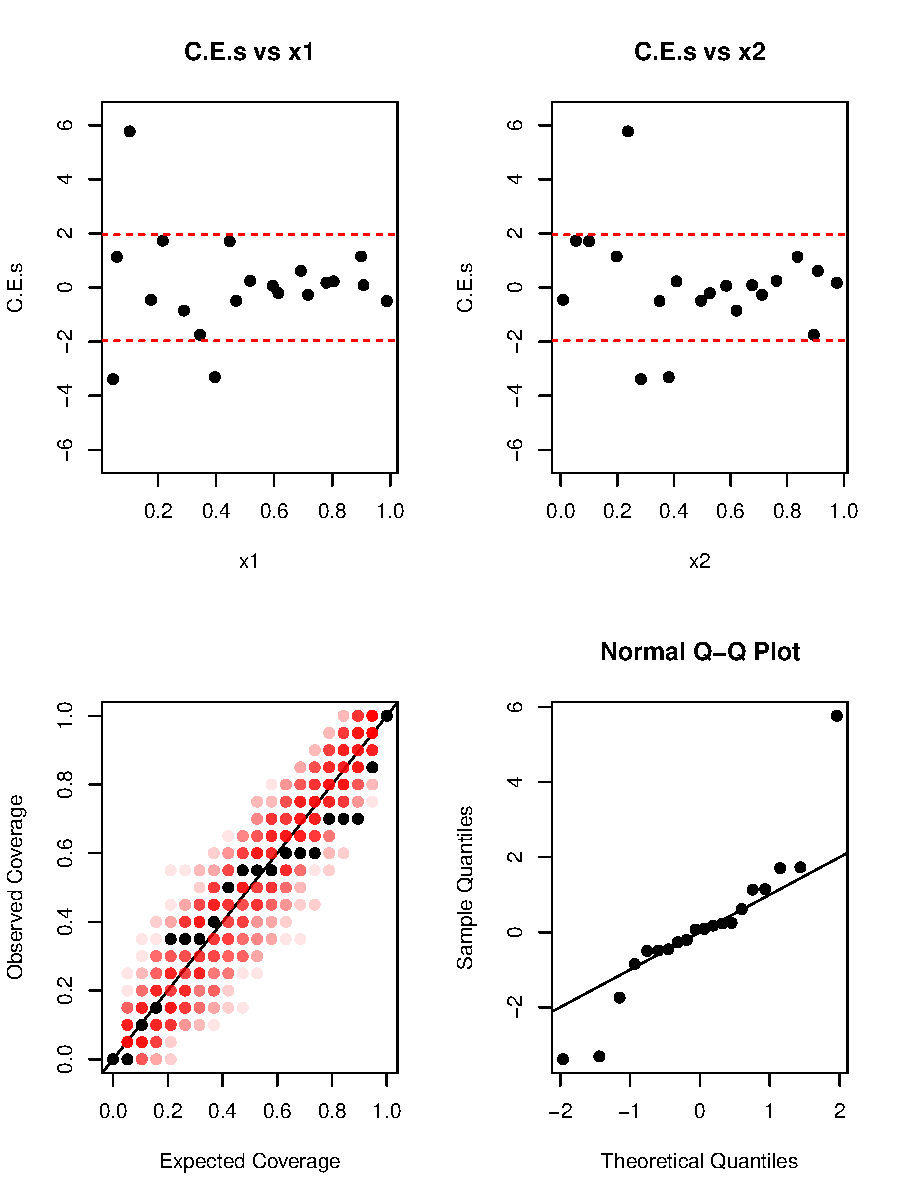
\includegraphics{fig-emulators/diags.pdf}
   \caption{Diagnostic Plots for the toy emulator. Top two plots are C.E.s against the inputs (left is input $1$, right is input $2$). Bottom right shows a QQ plot with the unit diagonal superimposed. Bottom left is the coverage plot, black points correspond to observed C.E.s, translucent red dots correspond to the coverage observed from $100$ iid $N(0,1)$ samples of size $20$.}
   \label{Fig:diags}
 \end{figure}
To improve the emulator we will follow BO'H and generate some additional data points and update the GP hyperparameters. If the simulator were very expensive this might not be possible. If further simulator runs are not possible, we can try other methods to improve the emulator. Common approaches include changing the mean function and/or covariance function to to better suit the training data \citep{Overstall2017, Volodina2020}.
We generate an additional $10$ points from an independent LH design on $(0, 0.5)^2$ in an attempt to build a satisfactory emulator. We update the hyperparameters to the values BO'H used; $\sigma^2 = 4.9389$, $\bm{\theta} =  (0.1764, 0.4116)$. The emulator is then refit leading to the diagnostics in \Cref{Fig:diag2}. The diagnostics are much improved; there are no very large C.E.s (we have one $|e_i|>1.96$, but this is expected in a sample of size $20$). There is no striking systematic pattern in the residuals, perhaps there is some indication of decreasing variance as the $x_i$ increase but this is hard to judge with a small sample size. The QQ-plot shows good fit to the line and the coverage plot is within the realms of what we would expect from a sample of size $20$.
\begin{figure}[H]
  \centering
  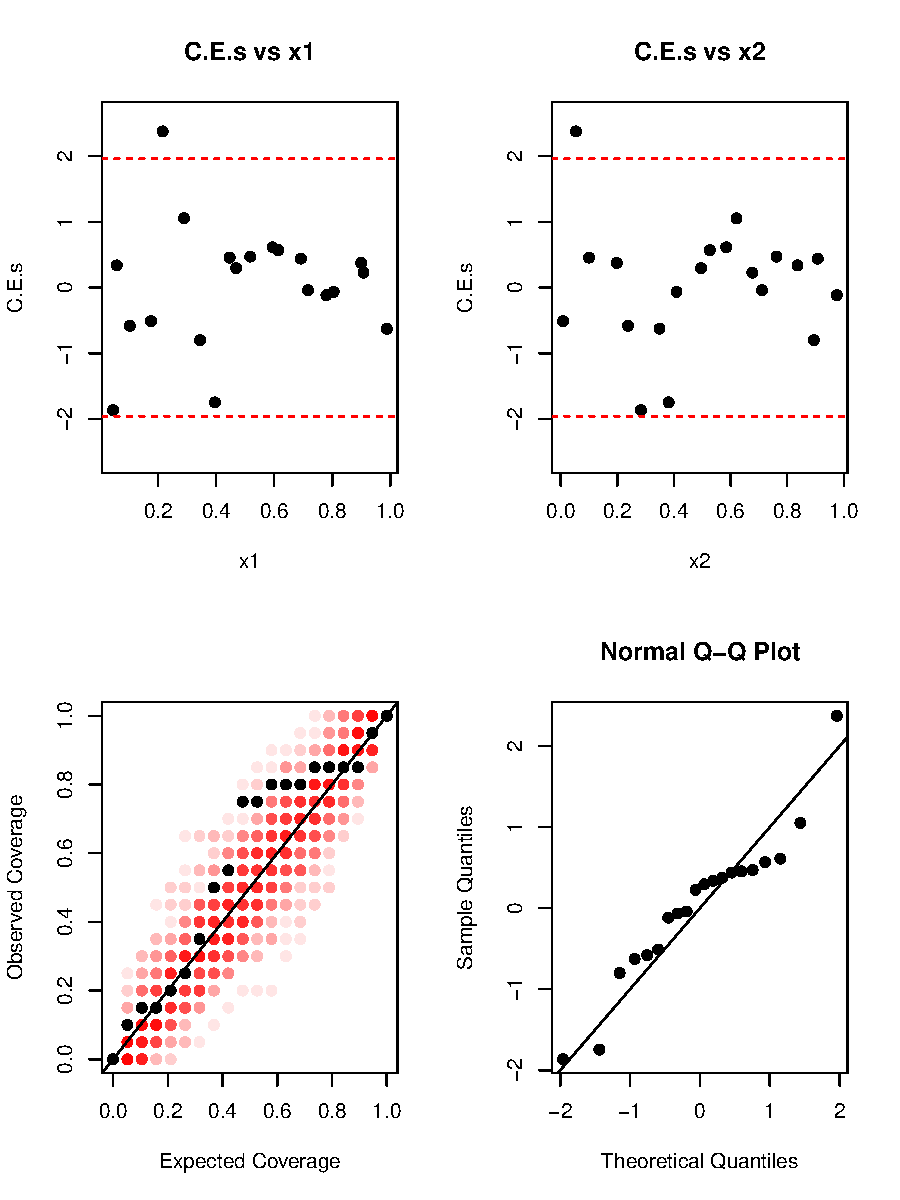
\includegraphics{fig-emulators/diag2.pdf}
  \caption{Diagnostic Plots for the toy emulator. Top two plots are C.E.s against the inputs (left is input $1$, right is input $2$). Bottom right shows a QQ plot with the unit diagonal superimposed. Bottom left is the coverage plot, black points correspond to observed C.E.s, translucent red dots correspond to the coverage observed from $100$ iid $N(0,1)$ samples of size $20$.}
  \label{Fig:diag2}
\end{figure}
\section{Other Surrogate Models}
Emulators do not have to be GPs. Other approaches have different advantages to GPs. For example, if the simulator inputs are permutations, the size of $||\bx - \bx'||$ implies little about $||f(\bx) - f(\bx')||$. In permutation space, a Benter model inspired emulator offers a promising solution \citep{Wilson2018}. Most non-GP surrogates do leverage some kind of smoothness about $f(\cdot)$ and thus re-purpose conventional regression techniques. Examples include generalised additive models, neural networks and splines \citep{Marrel2012, Tripathy2018, Barton2006}. We now discuss two non-GP emulators in turn.
\subsection{Linear Models}
Linear regression (Bayesian or frequentist) offers a much faster inference and prediction framework than GPs \citep{Rougier2009}. This is because GP inference relies on inverting a matrix, an $\mathcal{O}(n^3)$ operation. Prediction, given a GP precision matrix is then $\mathcal{O}(n^2)$. For fully Bayesian treatments with $S$ MCMC samples, predictions are typically $\mathcal{O}(S n^3)$, where S is fairly large ($S\approx10^4$). Inference is more costly still, in part to due mixing and thinning of MCMC schemes. For example, \citet{Baggaley2012} needed $550K$ MCMC iterations \textit{after} a series of trial MCMC schemes used to tune their sampling scheme. Under certain prior assumptions, the posterior distribution of a linear regression is fully tractable. One interpretation of the linear regression emulator is a type of emulator with a covariance that is ``all nugget''. The advantage of GPs over linear regression is that GPs automatically detect otherwise difficult to model features in the data, so the human cost of linear modelling -- fitting many different functional forms, including interaction and polynomial terms -- may be greater than the cost of inverting a matrix. The choice is between linear regression and GP is context dependent; \citet{Salter2016} explore this in detail and find merits in both approaches.
Although a simple approach, this can work quite well in both the stochastic and deterministic settings. For example, even when the simulator is deterministic, a nugget term is often incorporated. This might be a very small nugget for computational reasons or a larger nugget as a way to account for deviations from assumptions \citep{Gramacy12}. Another reason is that the fitted emulator might only depend on a subset of the variables fed into the simulator. This means that the emulator has a random component to account for the information `lost' by omitting unimportant variables from the emulator, thus a nugget is required almost always regardless of whether we have a stochastic or deterministic emulator.
\subsection{Bayes Linear Emulators}
Bayes Linear emulators \citep{Jones2016, Wilson18, Bower2010, Vernon2019} come from a framework which is, in principle, Bayesian. The prior specification is greatly simplified as the prior specification is only of means and (co)variances. In the Bayes Linear framework we want to update our beliefs about a vector of beliefs $B$ having observed a data vector $D$. Following \citet{BLS07} the ``posterior'' (known as \textit{adjusted}) mean and (co)variances are given by
\begin{align}
  \E_{D}(B) &= \E(B) + \cov(B, D) \var(D)^{-1}(D - \E(D)) \label{Eq:bl-mean}\\
  \var_{D}(B) & = \var(B) - \cov(B, D) \var(D)^{-1} \cov(D, B) \label{Eq:bl-var}.
\end{align}
These formulae bear a striking resemblance to the conditional Normal equations. Despite the resemblance, they have an important but subtle distinction from the conditional Normal equations. The conditional Normal equations are the posterior moments \textit{of a Normal distribution} and thus imply precise probability statements about $f(\bx)$. The Bayes Linear equations are distribution free statements (in terms of both the likelihood and prior) thus are not making precise probability statements. Proponents of a Bayes Linear analysis claim this simplified specification allows for a more robust analysis because we are not tied to probability statements. The downside is that it might be harder to interpret a Bayes Linear emulator. With a GP emulator, if $f(\bx) \sim N(0, 1)$ then we can make statements such as $\p (f(\bx)>0) = 0.5$, whereas a Bayes Linear emulator doesn't offer this level of detail. It is possible to make approximate probability statements by feeding the adjusted moments into certain results from probability theory such as Pukelsheim's $3\sigma$ rule \citet{Pukelsheim1994} or Markov's inequality. Neither approach is necessarily better, the advantages and disadvantages of each paradigm should be weighed up and it is indeed valid to mix the two approaches to leverage the benefits of each. One example of a mixed approach is \citet{Owen2020}; a (truncated) GP emulator and a Bayes Linear emulator are used together to emulate a simulator exhibiting $3$ behaviour patterns.
Ultimately, a Bayes Linear analysis produces a central estimate and quantification of uncertainty in an efficient way, which is all that is often needed from an emulator. A Bayes Linear analysis can be thought of as either an approximate Bayesian analysis or the appropriate analysis when we are only willing to specify means and (co)variances. Since \Cref{Eq:bl-mean} and \Cref{Eq:bl-var} are equivalent to \Cref{Eq:MV1} and \Cref{Eq:MV2} respectively.
In the Bayes Linear framework, we would usually take $D = y(X)$ and $B = y(X^*)$ (or $f(X^*)$) and $\cov(B, D)$ and $\var(D)$ can be found via assuming an appropriate covariance function, such as a squared exponential. This allows for a Bayesian emulator whilst avoiding MCMC schemes or other approximations. Although not strictly confined to the Bayes Linear framework necessary, proponents of the Bayes Linear framework typically use emulators of the form
\begin{equation}
  \hat{f}(\bx) = \sum_{j = 1}^q \beta_j h_j(\bx_{[A]}) + w(\bx_{[A]}) + \varepsilon(\bx)
\end{equation}
where $\bx_{[A]}$ are the ``active'' inputs, $\sum_{j = 1}^q \beta_j h_j(\bx_{[A]})$ is a mean function, $w(\cdot)$ is a mean-zero weakly stationary stochastic process and $\varepsilon(\cdot)$ is a white noise process. The mean function is often very detailed which means that there is a reduced reliance on choosing the correct form for $C(\cdot, \cdot)$. A more detailed mean function also allows the emulator to be more interpretable, as the regression coefficients are more understandable than the non-parametric component of the emulator \citep{Bower2010, Vernon2019}.
\section{Summary}
The purpose of this chapter was to motivate and establish the core concepts used later in the thesis. We began with the central concept of this thesis; an emulator. That is, a GP approximation to a simulator. We introduced the notion of a GP as a prior distribution over functions. We described how to encode certain prior beliefs about $f(\cdot)$ though this prior; we considered some common covariance structures for emulators and how these each imply different prior specifications for an unknown function. We also examined the effects of combining covariance structures. Multiplication of covariance structures typically leads to multiple input emulators; addition of covariance structures allows us to build emulators with different components.  We also discussed mean functions and evaluated the pros and cons of mean functions of different complexities.

We then moved to posterior inferences and design strategies for $f(\cdot)$. The multivariate Normal equations were presented as our path to an analytic posterior, conditional on GP hyperparameters; we discussed some approaches to estimation of both the hyperparameters and regression coefficients. We had a fleeting discussion of stochasticity; this will be greatly expanded upon in the next chapter. We contrasted one-shot and sequential designs and with a bias towards constructing space filling designs. \cref{Chap:optimisation} will discuss some sequential design approaches in greater detail with a particular emphasis on optimisation as a sequential problem.

The final GP emulator we considered in this chapter was an autoregressive emulator which used one cheap code level to improve both the emulation of a more expensive level of code, with a comparison to co-Kriging in geostatistics. We presented a concrete example of a two-level emulator but presented mathematical details of how to extend to an arbitrary number of levels. We then showed, via appropriate metrics, that the multilevel emulator out performed a standard emulator. We closed the consideration of GP emulators by presenting a suite of appropriate diagnostics for GP emulators.

We concluded this chapter on emulators by considering some approaches to emulation \textit{not} based on GPs. The first was linear regression based emulation, and the other was Bayes Linear emulation. Although both are different to GP emulation, they can both have strong links. Linear regression can be thought of as a GP emulator based on linear and white noise covariance functions. We saw that the multivariate Normal equations are mathematically identical to the Bayes Linear update equations.
\end{chapter}
